\documentclass{article}
% Shared style for the LUMEN manuscript diagrams (\input by every fig_*.tex; class: article).
% Uses only fonts and packages of a basic TeX installation (Computer Modern Sans), so compiling
% never triggers a package download. Each figure is wrapped in the lumenfig environment, which
% ships the picture out as a single page cropped to the drawing plus a 3 pt margin.
\usepackage{amsmath,amssymb}
\renewcommand{\familydefault}{\sfdefault}
\usepackage{tikz}
\usetikzlibrary{positioning,arrows.meta,fit,backgrounds,calc,shapes.geometric,decorations.pathreplacing}
\pagestyle{empty}

\newsavebox{\lumenfigbox}
\newenvironment{lumenfig}%
  {\begin{lrbox}{\lumenfigbox}}%
  {\end{lrbox}%
   \pdfpagewidth=\dimexpr\wd\lumenfigbox+6pt\relax
   \pdfpageheight=\dimexpr\ht\lumenfigbox+\dp\lumenfigbox+6pt\relax
   \hoffset=-1in\voffset=-1in
   \shipout\vbox{\kern3pt\hbox{\kern3pt\usebox{\lumenfigbox}}}}

% palette: physics (blue), learning (green), data (amber), reporting (violet), neutral ink
\definecolor{ink}{HTML}{1F2933}
\definecolor{muted}{HTML}{52606D}
\definecolor{rule}{HTML}{CBD2D9}
\definecolor{phyE}{HTML}{3B6EA8}\definecolor{phyF}{HTML}{E8F1FB}
\definecolor{lrnE}{HTML}{3C8C5A}\definecolor{lrnF}{HTML}{EAF6EE}
\definecolor{datE}{HTML}{B7791F}\definecolor{datF}{HTML}{FDF3E4}
\definecolor{outE}{HTML}{6B4FA0}\definecolor{outF}{HTML}{F3EEFB}
\definecolor{grey}{HTML}{9AA5B1}

\tikzset{
  >={Stealth[length=2.4mm,width=1.8mm]},
  every node/.style={font=\footnotesize, text=ink},
  box/.style={draw, rounded corners=2.5pt, line width=0.7pt, align=center, inner sep=4pt,
    execute at begin node={\hyphenpenalty=10000\exhyphenpenalty=10000}},
  phy/.style={box, draw=phyE, fill=phyF},
  lrn/.style={box, draw=lrnE, fill=lrnF},
  dat/.style={box, draw=datE, fill=datF},
  rep/.style={box, draw=outE, fill=outF},
  neutral/.style={box, draw=grey, fill=white},
  flow/.style={->, line width=0.8pt, draw=ink},
  soft/.style={->, line width=0.7pt, draw=muted, dashed},
  title/.style={font=\footnotesize\bfseries},
  note/.style={font=\scriptsize, text=muted, align=center},
  stage/.style={draw=rule, rounded corners=4pt, line width=0.6pt, dashed, inner sep=6pt},
  stagelabel/.style={font=\scriptsize\bfseries, text=muted, anchor=south west, inner sep=1pt},
}

\begin{document}
\begin{lumenfig}
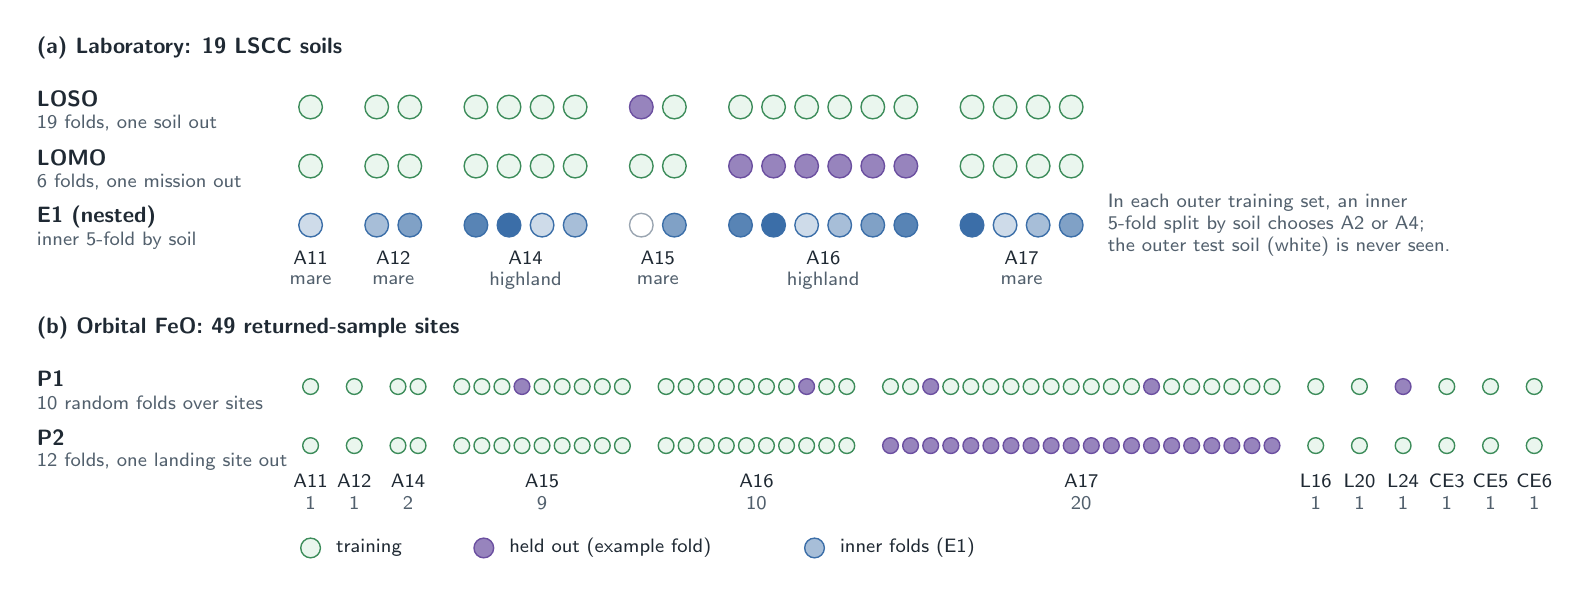
\begin{tikzpicture}
\node[title, anchor=west] at (0,0.75) {(a) Laboratory: 19 LSCC soils};
\node[anchor=west, font=\footnotesize\bfseries] at (0,0.10) {LOSO};
\node[anchor=west, note, align=left] at (0,-0.20) {19 folds, one soil out};
\node[circle, minimum size=0.30cm, inner sep=0pt, draw=lrnE, fill=lrnF, line width=0.5pt] at (3.600,-0.000) {};
\node[circle, minimum size=0.30cm, inner sep=0pt, draw=lrnE, fill=lrnF, line width=0.5pt] at (4.440,-0.000) {};
\node[circle, minimum size=0.30cm, inner sep=0pt, draw=lrnE, fill=lrnF, line width=0.5pt] at (4.860,-0.000) {};
\node[circle, minimum size=0.30cm, inner sep=0pt, draw=lrnE, fill=lrnF, line width=0.5pt] at (5.700,-0.000) {};
\node[circle, minimum size=0.30cm, inner sep=0pt, draw=lrnE, fill=lrnF, line width=0.5pt] at (6.120,-0.000) {};
\node[circle, minimum size=0.30cm, inner sep=0pt, draw=lrnE, fill=lrnF, line width=0.5pt] at (6.540,-0.000) {};
\node[circle, minimum size=0.30cm, inner sep=0pt, draw=lrnE, fill=lrnF, line width=0.5pt] at (6.960,-0.000) {};
\node[circle, minimum size=0.30cm, inner sep=0pt, draw=outE, fill=outE!70, line width=0.5pt] at (7.800,-0.000) {};
\node[circle, minimum size=0.30cm, inner sep=0pt, draw=lrnE, fill=lrnF, line width=0.5pt] at (8.220,-0.000) {};
\node[circle, minimum size=0.30cm, inner sep=0pt, draw=lrnE, fill=lrnF, line width=0.5pt] at (9.060,-0.000) {};
\node[circle, minimum size=0.30cm, inner sep=0pt, draw=lrnE, fill=lrnF, line width=0.5pt] at (9.480,-0.000) {};
\node[circle, minimum size=0.30cm, inner sep=0pt, draw=lrnE, fill=lrnF, line width=0.5pt] at (9.900,-0.000) {};
\node[circle, minimum size=0.30cm, inner sep=0pt, draw=lrnE, fill=lrnF, line width=0.5pt] at (10.320,-0.000) {};
\node[circle, minimum size=0.30cm, inner sep=0pt, draw=lrnE, fill=lrnF, line width=0.5pt] at (10.740,-0.000) {};
\node[circle, minimum size=0.30cm, inner sep=0pt, draw=lrnE, fill=lrnF, line width=0.5pt] at (11.160,-0.000) {};
\node[circle, minimum size=0.30cm, inner sep=0pt, draw=lrnE, fill=lrnF, line width=0.5pt] at (12.000,-0.000) {};
\node[circle, minimum size=0.30cm, inner sep=0pt, draw=lrnE, fill=lrnF, line width=0.5pt] at (12.420,-0.000) {};
\node[circle, minimum size=0.30cm, inner sep=0pt, draw=lrnE, fill=lrnF, line width=0.5pt] at (12.840,-0.000) {};
\node[circle, minimum size=0.30cm, inner sep=0pt, draw=lrnE, fill=lrnF, line width=0.5pt] at (13.260,-0.000) {};
\node[anchor=west, font=\footnotesize\bfseries] at (0,-0.65) {LOMO};
\node[anchor=west, note, align=left] at (0,-0.95) {6 folds, one mission out};
\node[circle, minimum size=0.30cm, inner sep=0pt, draw=lrnE, fill=lrnF, line width=0.5pt] at (3.600,-0.750) {};
\node[circle, minimum size=0.30cm, inner sep=0pt, draw=lrnE, fill=lrnF, line width=0.5pt] at (4.440,-0.750) {};
\node[circle, minimum size=0.30cm, inner sep=0pt, draw=lrnE, fill=lrnF, line width=0.5pt] at (4.860,-0.750) {};
\node[circle, minimum size=0.30cm, inner sep=0pt, draw=lrnE, fill=lrnF, line width=0.5pt] at (5.700,-0.750) {};
\node[circle, minimum size=0.30cm, inner sep=0pt, draw=lrnE, fill=lrnF, line width=0.5pt] at (6.120,-0.750) {};
\node[circle, minimum size=0.30cm, inner sep=0pt, draw=lrnE, fill=lrnF, line width=0.5pt] at (6.540,-0.750) {};
\node[circle, minimum size=0.30cm, inner sep=0pt, draw=lrnE, fill=lrnF, line width=0.5pt] at (6.960,-0.750) {};
\node[circle, minimum size=0.30cm, inner sep=0pt, draw=lrnE, fill=lrnF, line width=0.5pt] at (7.800,-0.750) {};
\node[circle, minimum size=0.30cm, inner sep=0pt, draw=lrnE, fill=lrnF, line width=0.5pt] at (8.220,-0.750) {};
\node[circle, minimum size=0.30cm, inner sep=0pt, draw=outE, fill=outE!70, line width=0.5pt] at (9.060,-0.750) {};
\node[circle, minimum size=0.30cm, inner sep=0pt, draw=outE, fill=outE!70, line width=0.5pt] at (9.480,-0.750) {};
\node[circle, minimum size=0.30cm, inner sep=0pt, draw=outE, fill=outE!70, line width=0.5pt] at (9.900,-0.750) {};
\node[circle, minimum size=0.30cm, inner sep=0pt, draw=outE, fill=outE!70, line width=0.5pt] at (10.320,-0.750) {};
\node[circle, minimum size=0.30cm, inner sep=0pt, draw=outE, fill=outE!70, line width=0.5pt] at (10.740,-0.750) {};
\node[circle, minimum size=0.30cm, inner sep=0pt, draw=outE, fill=outE!70, line width=0.5pt] at (11.160,-0.750) {};
\node[circle, minimum size=0.30cm, inner sep=0pt, draw=lrnE, fill=lrnF, line width=0.5pt] at (12.000,-0.750) {};
\node[circle, minimum size=0.30cm, inner sep=0pt, draw=lrnE, fill=lrnF, line width=0.5pt] at (12.420,-0.750) {};
\node[circle, minimum size=0.30cm, inner sep=0pt, draw=lrnE, fill=lrnF, line width=0.5pt] at (12.840,-0.750) {};
\node[circle, minimum size=0.30cm, inner sep=0pt, draw=lrnE, fill=lrnF, line width=0.5pt] at (13.260,-0.750) {};
\node[anchor=west, font=\footnotesize\bfseries] at (0,-1.40) {E1 (nested)};
\node[anchor=west, note, align=left] at (0,-1.70) {inner 5-fold by soil};
\node[circle, minimum size=0.30cm, inner sep=0pt, draw=phyE, fill=phyE!25, line width=0.5pt] at (3.600,-1.500) {};
\node[circle, minimum size=0.30cm, inner sep=0pt, draw=phyE, fill=phyE!45, line width=0.5pt] at (4.440,-1.500) {};
\node[circle, minimum size=0.30cm, inner sep=0pt, draw=phyE, fill=phyE!65, line width=0.5pt] at (4.860,-1.500) {};
\node[circle, minimum size=0.30cm, inner sep=0pt, draw=phyE, fill=phyE!85, line width=0.5pt] at (5.700,-1.500) {};
\node[circle, minimum size=0.30cm, inner sep=0pt, draw=phyE, fill=phyE, line width=0.5pt] at (6.120,-1.500) {};
\node[circle, minimum size=0.30cm, inner sep=0pt, draw=phyE, fill=phyE!25, line width=0.5pt] at (6.540,-1.500) {};
\node[circle, minimum size=0.30cm, inner sep=0pt, draw=phyE, fill=phyE!45, line width=0.5pt] at (6.960,-1.500) {};
\node[circle, minimum size=0.30cm, inner sep=0pt, draw=grey, fill=white, line width=0.5pt] at (7.800,-1.500) {};
\node[circle, minimum size=0.30cm, inner sep=0pt, draw=phyE, fill=phyE!65, line width=0.5pt] at (8.220,-1.500) {};
\node[circle, minimum size=0.30cm, inner sep=0pt, draw=phyE, fill=phyE!85, line width=0.5pt] at (9.060,-1.500) {};
\node[circle, minimum size=0.30cm, inner sep=0pt, draw=phyE, fill=phyE, line width=0.5pt] at (9.480,-1.500) {};
\node[circle, minimum size=0.30cm, inner sep=0pt, draw=phyE, fill=phyE!25, line width=0.5pt] at (9.900,-1.500) {};
\node[circle, minimum size=0.30cm, inner sep=0pt, draw=phyE, fill=phyE!45, line width=0.5pt] at (10.320,-1.500) {};
\node[circle, minimum size=0.30cm, inner sep=0pt, draw=phyE, fill=phyE!65, line width=0.5pt] at (10.740,-1.500) {};
\node[circle, minimum size=0.30cm, inner sep=0pt, draw=phyE, fill=phyE!85, line width=0.5pt] at (11.160,-1.500) {};
\node[circle, minimum size=0.30cm, inner sep=0pt, draw=phyE, fill=phyE, line width=0.5pt] at (12.000,-1.500) {};
\node[circle, minimum size=0.30cm, inner sep=0pt, draw=phyE, fill=phyE!25, line width=0.5pt] at (12.420,-1.500) {};
\node[circle, minimum size=0.30cm, inner sep=0pt, draw=phyE, fill=phyE!45, line width=0.5pt] at (12.840,-1.500) {};
\node[circle, minimum size=0.30cm, inner sep=0pt, draw=phyE, fill=phyE!65, line width=0.5pt] at (13.260,-1.500) {};
\node[note, text=ink] at (3.600,-1.92) {A11};
\node[note] at (3.600,-2.20) {mare};
\node[note, text=ink] at (4.650,-1.92) {A12};
\node[note] at (4.650,-2.20) {mare};
\node[note, text=ink] at (6.330,-1.92) {A14};
\node[note] at (6.330,-2.20) {highland};
\node[note, text=ink] at (8.010,-1.92) {A15};
\node[note] at (8.010,-2.20) {mare};
\node[note, text=ink] at (10.110,-1.92) {A16};
\node[note] at (10.110,-2.20) {highland};
\node[note, text=ink] at (12.630,-1.92) {A17};
\node[note] at (12.630,-2.20) {mare};
\node[note, anchor=west, align=left] at (13.60,-1.5) {In each outer training set, an inner\\5-fold split by soil chooses A2 or A4;\\the outer test soil (white) is never seen.};
\node[title, anchor=west] at (0,-2.80) {(b) Orbital FeO: 49 returned-sample sites};
\node[anchor=west, font=\footnotesize\bfseries] at (0,-3.45) {P1};
\node[anchor=west, note, align=left] at (0,-3.75) {10 random folds over sites};
\node[circle, minimum size=0.20cm, inner sep=0pt, draw=lrnE, fill=lrnF, line width=0.5pt] at (3.600,-3.550) {};
\node[circle, minimum size=0.20cm, inner sep=0pt, draw=lrnE, fill=lrnF, line width=0.5pt] at (4.155,-3.550) {};
\node[circle, minimum size=0.20cm, inner sep=0pt, draw=lrnE, fill=lrnF, line width=0.5pt] at (4.710,-3.550) {};
\node[circle, minimum size=0.20cm, inner sep=0pt, draw=lrnE, fill=lrnF, line width=0.5pt] at (4.965,-3.550) {};
\node[circle, minimum size=0.20cm, inner sep=0pt, draw=lrnE, fill=lrnF, line width=0.5pt] at (5.520,-3.550) {};
\node[circle, minimum size=0.20cm, inner sep=0pt, draw=lrnE, fill=lrnF, line width=0.5pt] at (5.775,-3.550) {};
\node[circle, minimum size=0.20cm, inner sep=0pt, draw=lrnE, fill=lrnF, line width=0.5pt] at (6.030,-3.550) {};
\node[circle, minimum size=0.20cm, inner sep=0pt, draw=outE, fill=outE!70, line width=0.5pt] at (6.285,-3.550) {};
\node[circle, minimum size=0.20cm, inner sep=0pt, draw=lrnE, fill=lrnF, line width=0.5pt] at (6.540,-3.550) {};
\node[circle, minimum size=0.20cm, inner sep=0pt, draw=lrnE, fill=lrnF, line width=0.5pt] at (6.795,-3.550) {};
\node[circle, minimum size=0.20cm, inner sep=0pt, draw=lrnE, fill=lrnF, line width=0.5pt] at (7.050,-3.550) {};
\node[circle, minimum size=0.20cm, inner sep=0pt, draw=lrnE, fill=lrnF, line width=0.5pt] at (7.305,-3.550) {};
\node[circle, minimum size=0.20cm, inner sep=0pt, draw=lrnE, fill=lrnF, line width=0.5pt] at (7.560,-3.550) {};
\node[circle, minimum size=0.20cm, inner sep=0pt, draw=lrnE, fill=lrnF, line width=0.5pt] at (8.115,-3.550) {};
\node[circle, minimum size=0.20cm, inner sep=0pt, draw=lrnE, fill=lrnF, line width=0.5pt] at (8.370,-3.550) {};
\node[circle, minimum size=0.20cm, inner sep=0pt, draw=lrnE, fill=lrnF, line width=0.5pt] at (8.625,-3.550) {};
\node[circle, minimum size=0.20cm, inner sep=0pt, draw=lrnE, fill=lrnF, line width=0.5pt] at (8.880,-3.550) {};
\node[circle, minimum size=0.20cm, inner sep=0pt, draw=lrnE, fill=lrnF, line width=0.5pt] at (9.135,-3.550) {};
\node[circle, minimum size=0.20cm, inner sep=0pt, draw=lrnE, fill=lrnF, line width=0.5pt] at (9.390,-3.550) {};
\node[circle, minimum size=0.20cm, inner sep=0pt, draw=lrnE, fill=lrnF, line width=0.5pt] at (9.645,-3.550) {};
\node[circle, minimum size=0.20cm, inner sep=0pt, draw=outE, fill=outE!70, line width=0.5pt] at (9.900,-3.550) {};
\node[circle, minimum size=0.20cm, inner sep=0pt, draw=lrnE, fill=lrnF, line width=0.5pt] at (10.155,-3.550) {};
\node[circle, minimum size=0.20cm, inner sep=0pt, draw=lrnE, fill=lrnF, line width=0.5pt] at (10.410,-3.550) {};
\node[circle, minimum size=0.20cm, inner sep=0pt, draw=lrnE, fill=lrnF, line width=0.5pt] at (10.965,-3.550) {};
\node[circle, minimum size=0.20cm, inner sep=0pt, draw=lrnE, fill=lrnF, line width=0.5pt] at (11.220,-3.550) {};
\node[circle, minimum size=0.20cm, inner sep=0pt, draw=outE, fill=outE!70, line width=0.5pt] at (11.475,-3.550) {};
\node[circle, minimum size=0.20cm, inner sep=0pt, draw=lrnE, fill=lrnF, line width=0.5pt] at (11.730,-3.550) {};
\node[circle, minimum size=0.20cm, inner sep=0pt, draw=lrnE, fill=lrnF, line width=0.5pt] at (11.985,-3.550) {};
\node[circle, minimum size=0.20cm, inner sep=0pt, draw=lrnE, fill=lrnF, line width=0.5pt] at (12.240,-3.550) {};
\node[circle, minimum size=0.20cm, inner sep=0pt, draw=lrnE, fill=lrnF, line width=0.5pt] at (12.495,-3.550) {};
\node[circle, minimum size=0.20cm, inner sep=0pt, draw=lrnE, fill=lrnF, line width=0.5pt] at (12.750,-3.550) {};
\node[circle, minimum size=0.20cm, inner sep=0pt, draw=lrnE, fill=lrnF, line width=0.5pt] at (13.005,-3.550) {};
\node[circle, minimum size=0.20cm, inner sep=0pt, draw=lrnE, fill=lrnF, line width=0.5pt] at (13.260,-3.550) {};
\node[circle, minimum size=0.20cm, inner sep=0pt, draw=lrnE, fill=lrnF, line width=0.5pt] at (13.515,-3.550) {};
\node[circle, minimum size=0.20cm, inner sep=0pt, draw=lrnE, fill=lrnF, line width=0.5pt] at (13.770,-3.550) {};
\node[circle, minimum size=0.20cm, inner sep=0pt, draw=lrnE, fill=lrnF, line width=0.5pt] at (14.025,-3.550) {};
\node[circle, minimum size=0.20cm, inner sep=0pt, draw=outE, fill=outE!70, line width=0.5pt] at (14.280,-3.550) {};
\node[circle, minimum size=0.20cm, inner sep=0pt, draw=lrnE, fill=lrnF, line width=0.5pt] at (14.535,-3.550) {};
\node[circle, minimum size=0.20cm, inner sep=0pt, draw=lrnE, fill=lrnF, line width=0.5pt] at (14.790,-3.550) {};
\node[circle, minimum size=0.20cm, inner sep=0pt, draw=lrnE, fill=lrnF, line width=0.5pt] at (15.045,-3.550) {};
\node[circle, minimum size=0.20cm, inner sep=0pt, draw=lrnE, fill=lrnF, line width=0.5pt] at (15.300,-3.550) {};
\node[circle, minimum size=0.20cm, inner sep=0pt, draw=lrnE, fill=lrnF, line width=0.5pt] at (15.555,-3.550) {};
\node[circle, minimum size=0.20cm, inner sep=0pt, draw=lrnE, fill=lrnF, line width=0.5pt] at (15.810,-3.550) {};
\node[circle, minimum size=0.20cm, inner sep=0pt, draw=lrnE, fill=lrnF, line width=0.5pt] at (16.365,-3.550) {};
\node[circle, minimum size=0.20cm, inner sep=0pt, draw=lrnE, fill=lrnF, line width=0.5pt] at (16.920,-3.550) {};
\node[circle, minimum size=0.20cm, inner sep=0pt, draw=outE, fill=outE!70, line width=0.5pt] at (17.475,-3.550) {};
\node[circle, minimum size=0.20cm, inner sep=0pt, draw=lrnE, fill=lrnF, line width=0.5pt] at (18.030,-3.550) {};
\node[circle, minimum size=0.20cm, inner sep=0pt, draw=lrnE, fill=lrnF, line width=0.5pt] at (18.585,-3.550) {};
\node[circle, minimum size=0.20cm, inner sep=0pt, draw=lrnE, fill=lrnF, line width=0.5pt] at (19.140,-3.550) {};
\node[anchor=west, font=\footnotesize\bfseries] at (0,-4.20) {P2};
\node[anchor=west, note, align=left] at (0,-4.50) {12 folds, one landing site out};
\node[circle, minimum size=0.20cm, inner sep=0pt, draw=lrnE, fill=lrnF, line width=0.5pt] at (3.600,-4.300) {};
\node[circle, minimum size=0.20cm, inner sep=0pt, draw=lrnE, fill=lrnF, line width=0.5pt] at (4.155,-4.300) {};
\node[circle, minimum size=0.20cm, inner sep=0pt, draw=lrnE, fill=lrnF, line width=0.5pt] at (4.710,-4.300) {};
\node[circle, minimum size=0.20cm, inner sep=0pt, draw=lrnE, fill=lrnF, line width=0.5pt] at (4.965,-4.300) {};
\node[circle, minimum size=0.20cm, inner sep=0pt, draw=lrnE, fill=lrnF, line width=0.5pt] at (5.520,-4.300) {};
\node[circle, minimum size=0.20cm, inner sep=0pt, draw=lrnE, fill=lrnF, line width=0.5pt] at (5.775,-4.300) {};
\node[circle, minimum size=0.20cm, inner sep=0pt, draw=lrnE, fill=lrnF, line width=0.5pt] at (6.030,-4.300) {};
\node[circle, minimum size=0.20cm, inner sep=0pt, draw=lrnE, fill=lrnF, line width=0.5pt] at (6.285,-4.300) {};
\node[circle, minimum size=0.20cm, inner sep=0pt, draw=lrnE, fill=lrnF, line width=0.5pt] at (6.540,-4.300) {};
\node[circle, minimum size=0.20cm, inner sep=0pt, draw=lrnE, fill=lrnF, line width=0.5pt] at (6.795,-4.300) {};
\node[circle, minimum size=0.20cm, inner sep=0pt, draw=lrnE, fill=lrnF, line width=0.5pt] at (7.050,-4.300) {};
\node[circle, minimum size=0.20cm, inner sep=0pt, draw=lrnE, fill=lrnF, line width=0.5pt] at (7.305,-4.300) {};
\node[circle, minimum size=0.20cm, inner sep=0pt, draw=lrnE, fill=lrnF, line width=0.5pt] at (7.560,-4.300) {};
\node[circle, minimum size=0.20cm, inner sep=0pt, draw=lrnE, fill=lrnF, line width=0.5pt] at (8.115,-4.300) {};
\node[circle, minimum size=0.20cm, inner sep=0pt, draw=lrnE, fill=lrnF, line width=0.5pt] at (8.370,-4.300) {};
\node[circle, minimum size=0.20cm, inner sep=0pt, draw=lrnE, fill=lrnF, line width=0.5pt] at (8.625,-4.300) {};
\node[circle, minimum size=0.20cm, inner sep=0pt, draw=lrnE, fill=lrnF, line width=0.5pt] at (8.880,-4.300) {};
\node[circle, minimum size=0.20cm, inner sep=0pt, draw=lrnE, fill=lrnF, line width=0.5pt] at (9.135,-4.300) {};
\node[circle, minimum size=0.20cm, inner sep=0pt, draw=lrnE, fill=lrnF, line width=0.5pt] at (9.390,-4.300) {};
\node[circle, minimum size=0.20cm, inner sep=0pt, draw=lrnE, fill=lrnF, line width=0.5pt] at (9.645,-4.300) {};
\node[circle, minimum size=0.20cm, inner sep=0pt, draw=lrnE, fill=lrnF, line width=0.5pt] at (9.900,-4.300) {};
\node[circle, minimum size=0.20cm, inner sep=0pt, draw=lrnE, fill=lrnF, line width=0.5pt] at (10.155,-4.300) {};
\node[circle, minimum size=0.20cm, inner sep=0pt, draw=lrnE, fill=lrnF, line width=0.5pt] at (10.410,-4.300) {};
\node[circle, minimum size=0.20cm, inner sep=0pt, draw=outE, fill=outE!70, line width=0.5pt] at (10.965,-4.300) {};
\node[circle, minimum size=0.20cm, inner sep=0pt, draw=outE, fill=outE!70, line width=0.5pt] at (11.220,-4.300) {};
\node[circle, minimum size=0.20cm, inner sep=0pt, draw=outE, fill=outE!70, line width=0.5pt] at (11.475,-4.300) {};
\node[circle, minimum size=0.20cm, inner sep=0pt, draw=outE, fill=outE!70, line width=0.5pt] at (11.730,-4.300) {};
\node[circle, minimum size=0.20cm, inner sep=0pt, draw=outE, fill=outE!70, line width=0.5pt] at (11.985,-4.300) {};
\node[circle, minimum size=0.20cm, inner sep=0pt, draw=outE, fill=outE!70, line width=0.5pt] at (12.240,-4.300) {};
\node[circle, minimum size=0.20cm, inner sep=0pt, draw=outE, fill=outE!70, line width=0.5pt] at (12.495,-4.300) {};
\node[circle, minimum size=0.20cm, inner sep=0pt, draw=outE, fill=outE!70, line width=0.5pt] at (12.750,-4.300) {};
\node[circle, minimum size=0.20cm, inner sep=0pt, draw=outE, fill=outE!70, line width=0.5pt] at (13.005,-4.300) {};
\node[circle, minimum size=0.20cm, inner sep=0pt, draw=outE, fill=outE!70, line width=0.5pt] at (13.260,-4.300) {};
\node[circle, minimum size=0.20cm, inner sep=0pt, draw=outE, fill=outE!70, line width=0.5pt] at (13.515,-4.300) {};
\node[circle, minimum size=0.20cm, inner sep=0pt, draw=outE, fill=outE!70, line width=0.5pt] at (13.770,-4.300) {};
\node[circle, minimum size=0.20cm, inner sep=0pt, draw=outE, fill=outE!70, line width=0.5pt] at (14.025,-4.300) {};
\node[circle, minimum size=0.20cm, inner sep=0pt, draw=outE, fill=outE!70, line width=0.5pt] at (14.280,-4.300) {};
\node[circle, minimum size=0.20cm, inner sep=0pt, draw=outE, fill=outE!70, line width=0.5pt] at (14.535,-4.300) {};
\node[circle, minimum size=0.20cm, inner sep=0pt, draw=outE, fill=outE!70, line width=0.5pt] at (14.790,-4.300) {};
\node[circle, minimum size=0.20cm, inner sep=0pt, draw=outE, fill=outE!70, line width=0.5pt] at (15.045,-4.300) {};
\node[circle, minimum size=0.20cm, inner sep=0pt, draw=outE, fill=outE!70, line width=0.5pt] at (15.300,-4.300) {};
\node[circle, minimum size=0.20cm, inner sep=0pt, draw=outE, fill=outE!70, line width=0.5pt] at (15.555,-4.300) {};
\node[circle, minimum size=0.20cm, inner sep=0pt, draw=outE, fill=outE!70, line width=0.5pt] at (15.810,-4.300) {};
\node[circle, minimum size=0.20cm, inner sep=0pt, draw=lrnE, fill=lrnF, line width=0.5pt] at (16.365,-4.300) {};
\node[circle, minimum size=0.20cm, inner sep=0pt, draw=lrnE, fill=lrnF, line width=0.5pt] at (16.920,-4.300) {};
\node[circle, minimum size=0.20cm, inner sep=0pt, draw=lrnE, fill=lrnF, line width=0.5pt] at (17.475,-4.300) {};
\node[circle, minimum size=0.20cm, inner sep=0pt, draw=lrnE, fill=lrnF, line width=0.5pt] at (18.030,-4.300) {};
\node[circle, minimum size=0.20cm, inner sep=0pt, draw=lrnE, fill=lrnF, line width=0.5pt] at (18.585,-4.300) {};
\node[circle, minimum size=0.20cm, inner sep=0pt, draw=lrnE, fill=lrnF, line width=0.5pt] at (19.140,-4.300) {};
\node[note, text=ink] at (3.600,-4.75) {A11};
\node[note] at (3.600,-5.03) {1};
\node[note, text=ink] at (4.155,-4.75) {A12};
\node[note] at (4.155,-5.03) {1};
\node[note, text=ink] at (4.838,-4.75) {A14};
\node[note] at (4.838,-5.03) {2};
\node[note, text=ink] at (6.540,-4.75) {A15};
\node[note] at (6.540,-5.03) {9};
\node[note, text=ink] at (9.262,-4.75) {A16};
\node[note] at (9.262,-5.03) {10};
\node[note, text=ink] at (13.387,-4.75) {A17};
\node[note] at (13.387,-5.03) {20};
\node[note, text=ink] at (16.365,-4.75) {L16};
\node[note] at (16.365,-5.03) {1};
\node[note, text=ink] at (16.920,-4.75) {L20};
\node[note] at (16.920,-5.03) {1};
\node[note, text=ink] at (17.475,-4.75) {L24};
\node[note] at (17.475,-5.03) {1};
\node[note, text=ink] at (18.030,-4.75) {CE3};
\node[note] at (18.030,-5.03) {1};
\node[note, text=ink] at (18.585,-4.75) {CE5};
\node[note] at (18.585,-5.03) {1};
\node[note, text=ink] at (19.140,-4.75) {CE6};
\node[note] at (19.140,-5.03) {1};
\node[circle, minimum size=0.25cm, inner sep=0pt, draw=lrnE, fill=lrnF, line width=0.5pt] at (3.600,-5.600) {};
\node[note, text=ink, anchor=west] at (3.80,-5.60) {training};
\node[circle, minimum size=0.25cm, inner sep=0pt, draw=outE, fill=outE!70, line width=0.5pt] at (5.800,-5.600) {};
\node[note, text=ink, anchor=west] at (6.00,-5.60) {held out (example fold)};
\node[circle, minimum size=0.25cm, inner sep=0pt, draw=phyE, fill=phyE!45, line width=0.5pt] at (10.000,-5.600) {};
\node[note, text=ink, anchor=west] at (10.20,-5.60) {inner folds (E1)};
\end{tikzpicture}
\end{lumenfig}
\end{document}
